\documentclass[utf8]{gradu3}
% Jos työ on kandidaatintutkielma eikä pro gradu, käytä ylläolevan asemesta
%\documentclass[utf8,bachelor]{gradu3}
% Jos kirjoitat englanniksi, käytä ylläolevan asemesta
%\documentclass[utf8,english]{gradu3}
% tai
%\documentclass[utf8,bachelor,english]{gradu3}

\usepackage{graphicx} % kuvien mukaan ottamista varten

\usepackage{amsmath} % hyödyllinen jos tekstisi sisältää matikkaa,
                     % ei pakollinen

\usepackage{booktabs} % hyvä kauniiden taulukoiden tekemiseen
\usepackage{listings}
\usepackage{color}
\usepackage{qtree}

% HUOM! Tämän tulee olla viimeinen \usepackage koko dokumentissa!
\usepackage[bookmarksopen,bookmarksnumbered,linktocpage]{hyperref}

\addbibresource{thesis.bib} % Lähdetietokannan tiedostonimi

\definecolor{light-gray}{gray}{0.96}

\lstdefinelanguage{Smalltalk}{
morekeywords={true,false,self,super,nil},
sensitive=true,
morecomment=[s][\color{blue}]{"}{"},
morestring=[d]',
alsoother={_},
style=SmalltalkStyle,
columns=fullflexible,
backgroundcolor=\color{light-gray},
xleftmargin=.20in,
showspaces=false,
numbers=left,
framexleftmargin=15pt,
tabsize=4
}
\lstdefinestyle{SmalltalkStyle}{
literate={:=}{{$\gets\ $}}2{^}{{$\uparrow$}}1{_}{{$\gets\ $}}2{ä}{{\"a}}2{ö}{{\"o}}2
}


\begin{document}

\title{\LaTeX-tutkielmapohjan {gradu3} käyttö}
\translatedtitle{Usage of the {gradu3} document class for \LaTeX\ theses}
\studyline{Kaikki suuntautumisvaihtoehdot}
\avainsanat{%
  \LaTeX,
  {gradu3},
  pro gradu -tutkielmat,
  kandidaatintutkielmat,
  käyttöohje}
\keywords{\LaTeX, {gradu3}, Master's Theses, Bachelor's Theses, user's guide}
\tiivistelma{%
  Tämä kirjoitelma on esimerkki siitä, kuinka
  {gradu3}-tutkielmapohjaa käytetään.  Se sisältää myös
  käyttöohjeet ja tutkielman rakennetta koskevia ohjeita.

  Tutkielman tiivistelmä on tyypillisesti lyhyt esitys, jossa
  kerrotaan tutkielman taustoista, tavoitteesta, tutkimusmenetelmistä,
  saavutetuista tuloksista, tulosten tulkinnasta ja johtopäätöksistä.
  Tiivistelmän tulee olla niin lyhyt, että se, englanninkielinen
  abstrakti ja muut metatiedot mahtuvat kaikki samalle sivulle.
}
\abstract{%
  This document is a sample {gradu3} thesis document class
  document.  It also functions as a user manual and supplies
  guidelines for structuring a thesis document.

  The English abstract of a thesis should usually say exactly the same
  things as the Finnish tiivistelmä.
}

\author{Antti-Juhani Kaijanaho}
\contactinformation{Ag~C416.1, \texttt{antti-juhani.kaijanaho@jyu.fi}}
% jos useita tekijöitä, anna useampi \author-komento
\supervisor{Ohjaamaton työ}
% jos useita ohjaajia, anna useampi \supervisor-komento

\type{tutkielmapohjan esimerkki ja käsikirja} % et tarvitse tätä riviä tutkielmassa!

\maketitle

\preface
Tähän voit kirjoittaa tutkielmasi esipuheen.  Tutkielmissa on
harvemmin esipuheita, mutta jos sen kirjoitat, pidä se lyhyenä
(enintään sivu).

Esipuheen tulisi kertoa ennemminkin tutkielmaprosessista kuin
tutkielman sisällöstä.  Esimerkiksi jos tutkielman aiheen valintaan
tai tekemiseen liittyy jokin erikoinen sattumus, voit siitä kertoa
esipuheessa.  Tapana esipuheessa on myös kiittää nimeltä mainiten
tärkeimpiä tutkielman tekemisessä auttaneita ihmisiä -- ainakin
ohjaajia, puolisoa ja lapsia.  (Yleensä perhe on auttanut vähintään
tukemalla ja kannustamalla.)

Esipuhe kannattaa kirjoittaa minä-muodossa. Tavanomaista on myös
allekirjoittaa se.

Jyväskylässä \today

\bigskip

Tutkielman tekijä


\begin{thetermlist}
\item[Sovellusarkkitehtuuri] Donald Knuthin 1977--1989 laatima eräajotyyppinenj
  ladontajärjestelmä \parencite[ks.][]{knuth86:_texbook}. 
\item[MVC] \TeX in \parencite[ks.][]{knuth86:_texbook} päälle
  rakennettu rakenteisten kirjoitelmien ladontaan tarkoitettu
  järjestelmä \parencite[ks.][]{lamport94:_latex}.  Siitä on nykyään
  käytössä versio \LaTeXe.
\item[Sovelluskehys] \TeX in \parencite[ks.][]{knuth86:_texbook} päälle
  rakennettu rakenteisten kirjoitelmien ladontaan tarkoitettu
  järjestelmä \parencite[ks.][]{lamport94:_latex}.  Siitä on nykyään
  käytössä versio \LaTeXe.
\item[WSGI] määrittää miten web-palvelin kommunikoi web-sovellusten kanssa ja millä tavalla web-sovellukset
yhdistetään prosessoimaan pyyntöjä.
\item[Myghty Python Templating Framework] \TeX in \parencite[ks.][]{knuth86:_texbook} päälle
  rakennettu rakenteisten kirjoitelmien ladontaan tarkoitettu
  järjestelmä \parencite[ks.][]{lamport94:_latex}.  Siitä on nykyään
  käytössä versio \LaTeXe.
\item[mod\_python] \TeX in \parencite[ks.][]{knuth86:_texbook} päälle
  rakennettu rakenteisten kirjoitelmien ladontaan tarkoitettu
  järjestelmä \parencite[ks.][]{lamport94:_latex}.  Siitä on nykyään
  käytössä versio \LaTeXe.
\item[BFG] \TeX in \parencite[ks.][]{knuth86:_texbook} päälle
  rakennettu rakenteisten kirjoitelmien ladontaan tarkoitettu
  järjestelmä \parencite[ks.][]{lamport94:_latex}.  Siitä on nykyään
  käytössä versio \LaTeXe.
\end{thetermlist}

\chapter{Johdanto}

\section{Tausta}
\section{Tutkimuskysymys}
MVC-arkkitehtuuri on saanut paljon huomiota web-sovelluskehyksien
toteutuksissa ja useat web-sovelluskehykset ovat luokiteltu
MVC-pohjaisiksi sovelluskehyksiksi \parencite{mvcframeworks}. Se on kuitenkin alunperin
tarkoitettu matalan tason käyttöliittymäsovellusten toteuttamiseen,
jossa esimerkiksi hallitaan yksittäisiä näppäimistöltä tulleita
syötteitä eikä sitä ole suoraan tarkoitettu käytettäväksi
web-sovellusten ohjelmointiin. Alkuperäisen MVC:n toteutuksen
soveltuvuutta web-ohjelmointiin onkin epäilty. Esimerkiksi Leff
soveltaa artikkelissaan MVC:n käyttämistä web-sovelluksissa, mutta
samalla esittelee alkuperäisen MVC:n toteuttamisen ongelmana. Tämä johtuu web-sovelluksen jakautumisesta asiakkaan
(client) ja palvelimen (server) välille \parencite{ibm_watson}. Myös Pyramid-sovelluskehyksen tekijät
kyseenalaistavat MVC-arkkitehtuurin toteutuksen Pyramidissa ja uskovat
MVC:n olevan sellaisenaan sopimaton web-ohjelmointiin, vaikka
Pyramidin toteutus onkin hyvin lähellä alkuperäistä MVC:tä
\parencite{pyramid}. Django on myös toteutettu MVC:n pohjalta, mutta
se ei kuitenkaan toteuta MVC:tä sellaisenaan \parencite{django}.

Tutkimuksen tarkoituksena on selvittää millä tavalla
MVC-arkkitehtuuri on toteutettu web-sovelluskehyksissä ja miten se
eroaa alkuperäisestä MVC:n toteutuksesta. Lisäksi laajennetaan
Flask-sovelluskehys toteuttamaan alkuperäinen MVC niinkuin Krasner on
sen määritellyt \parencite{krasner}. Havaintojen pohjalta
selvitetään voidaanko MVC tuoda sellaisenaan sovelluskehykseen ja
mitä mahdollisia ongelmia se tuo.

\chapter{Oletus}
Tutkimustulokseksi oletetaan, että MVC:tä ei sellaisenaan voida tuoda web-sovelluskehykseen. Oletus perustuu ohjaimen
konkreettiseen puuttumiseen sekä viestejen toteutukseen.

\chapter{Tutkimuksen Rakenne}
Tutkimus aloitetaan kirjallisuuskatsauksella, jossa tarkastellaan mitä aiempaa 
tutkimusta MVC:stä on tehty. Lisäksi käydään
läpi mitä lähteitä löytyy Python-pohjaisista web-sovelluskehyksistä. Tämän jälkeen 
tutkitaan MVC:n historiaa sekä millä tavalla MVC on tarkoitettu toteutettavaksi.
Tässä vaiheessa käydään läpi jokaisen MVC-komponentin tarkoitus sekä niiden 
keskinäisen kommunikaation rakentuminen. Lisäksi esitellään
Dortmundin yliopistossa kirjoitettu esimerkkiohjelma Smalltalkilla siitä miten MVC:n 
toteutus tuodaan sovellukseen käytännössä.

MVC:n tarkastelun jälkeen esitellään tutkimuksessa käytetyt web-sovelluskehykset, 
joita käytetään apuna MVC:n tutkimisessa. Sovelluskehyksistä käydään läpi sen 
historia sekä yleisellä tasolla mihin käyttötarkoitukseen
sovelluskehys on tarkoitettu. Tämän jälkeen verrataan MVC:n toteutusta erikseen 
jokaiseen sovelluskehykseen ja selvitetään millä tavalla niiden sovellusarkkitehtuuri 
mahdollisesti eroaa MVC:stä,
Havaintojen perusteella pohditaan MVC:n mahdollisia ongelmia sovelluskehyksien toteutuksessa 
ja selvitetään löytyykö sovelluskehyksien arkkitehtuurista jotain yhtenäisiä piirteitä, mitkä ovat
kytköksissä MVC:n toteutukseen. Saatujen tulosten pohjalta  kirjoitetaan Flask-sovellus, joka toteuttaa MVC:n 
niinkuin se on alunperin tarkoitettu.

Tutkimuksen lopuksi koostetaan havainnoista yhteenveto, jossa pohditaan saatuja tuloksia ja selvitetään 
pystytäänkö niiden perusteella vastaamaan tutkimuskysymykseen.


\section{Aiheen rajaus}
Tutkimus on rajattu tarkastelemaan MVC-arkkitehtuurin
toteutusta Pythonilla kirjoitetuissa
web-sovelluskehyksissä. Tarkasteltavat web-sovelluskehykset rajataan 
Pyramid-, Django-, Plone- sekä Flask-sovelluskehyksiin. Pyramid, Django ja Plone toteuttavat MVC:n kaltaisen
sovellusarkkitehtuurin. Flask on sovelluskehys, joka tarjoaa vain
välttämättömät kirjastot web-sovelluksen toteuttamiseen. Sitä
käytetään tutkimuksessa työkaluna selvittämään miten MVC tulisi
toteuttaa sovelluskehykseen. MVC:stä on olemassa erilaisia versioita, joten sen määrittely tulee rajata tarkasti.
Kun puhutaan MVC:stä tarkoitetaan tällä Krasnerin
artikkelissa esiteltyjä määrittelyitä MVC:n
toteutuksesta \parencite{krasner}, jotka pohjautuvat Trygve Reenskaugin esittelemään 
MVC:n määritelmään \parencite{xerox-original}. 

Tarkasteltavat sovelluskehykset käydään ensiksi yleisellä tasolla läpi, jonka jälkeen niitä tarkastellaan MVC:n näkökulmasta. Yleisellä tasolla tarkoitetaan sovelluskehyksen historian ja käyttötarkoituksen esittelemistä. Sovelluskehyksien muihin teknisiin ominaisuuksiin ei oteta kantaa. Flask-osiossa MVC-arkkitehtuuri toteutaan niinkuin se on Krasnerin julkaisussa määritelty. Näiden havaintojen pohjalta pyritään vastamaan tutkimuskysymykseen.


\chapter{Kirjallisuuskatsaus}
\section{Toteutus}
Kirjallisuuskatsauksessa käydään läpi vaihe vaiheelta, miten
lähdemateriaalia kerätään tutkimusta varten. Lähdemateriaalin 
haku toteutetaan hakukoneilla, jotka ovat tarkoitettu erityisesti 
tieteellisten artikkeleiden etsimiseen. Tässä tutkielmassa käytetyt 
hakukoneet ovat seuraavat: IEEE Xplore, ACM Digital Library, 
Google Scholar sekä joissakin tapauksissa Google:n yleinen
hakukone. Yleistä hakukonetta on käytetty esimerkiksi
sovelluskehyksien dokumentaatioiden etsintään.

Aluksi muodostetaan kokonaiskuva tuloksista, jolloin silmäillään läpi
saatuja artikkeleita. Tässä vaiheessa tarkoitus ei ole vielä valita
mitään pohjaksi tutkielmalle, vaan kerätä informaatiota siitä
millainen lähdemateriaali on tarjolla kokonaisuudessaan. Saaduista 
tuloksista poimitaan artikkeleita, jotka sopivat tutkimuksen aihepiiriin.
Seuraavaksi artikkeleista valitaan tutkielmalle
pohjakirjallisuus. Tässä vaiheessa artikkelit luetaan huolellisesti
läpi ja varmistutaan siitä, että ne ovat tieteellisesti päteviä
tutkielmaa varten. Erityisesti kiinnitetään huomiota viittauksien
määrän valittaessa tärkeimmät lähdemateriaalit. Tutkielmassa esiintyy myös satunnaisia viittauksia,
joita ei ole kirjallisuuskatsauksessa mainittu. Tutkimuksen
pääkirjallisuus kuitenkin käydään läpi kirjallisuuskatsauksessa.
Haussa käytetään seuraavia hakutermejä: "MVC", "MVC Architecture",
"frameworks", "web frameworks" ja  "MVC- Architecture". Erityisesti artikkeleita löytyy
MVC-arkkitehtuurin soveltamisesta erilaisissa
tekniikoissa. Tarkasteltavat artikkelit rajataan kuitenkin niihin,
jotka esittelevät suoraan MVC:tä itseään tai tarjoavat
lähdemateriaalin sovelluskehyksien esittelyyn.

\section{MVC}
Google Scholarin tuloksista löytyy kolme artikkelia MVC:stä, jotka sopivat 
lähdemateriaaliksi tutkimukseen. Ensimmäinen artikkeleista on John
Deaconin  kirjoittama artikkeli, joka tarkastelee lyhyesti
MVC:tä \parencite{deacon}. Artikkeli on kuitenkin hyvin suppea, mutta selittää
tiivistetysti MVC:n idean. Toinen artikkeli on Steve Burbeckin kirjoittama, 
joka käsittelee
MVC:tä sellaisena kuin sitä käytettiin Smalltalkissa \parencite{burbeck}. Burbeckin
artikkeliin viitataan monissa MVC:tä käsittelevissä
julkaisuissa, joten sen arvo tämän tutkielman pohjakirjallisuudessa on
vahva. Viittausten määrä on katsottu hakemalla artikkelia Google
Scholarin hakukoneessa. Viittauksia kyseiseen artikkeliin on
kirjoitushetkellä 308. Seuraavaksi kartoitetaan pohjakirjallisuutta käyttäen ACM Digital
Library sekä IEEE XPlore -hakukoneita. Kolmas artikkeli Glenn
E. Krasnerin kirjoittama julkaisu, jossa esitellään MVC:n toteutusta
erilaisissa Smalltalk-sovelluksissa. Julkaisusta löytyy useita
versioita, joista tässä tutkielmassa käytetään
molempia \parencite{krasner} \parencite[krasner_desc]. Tähän artikkeliin on
myös viitattu runsaasti, joten se on Burbeckin julkaisun kanssa
tärkeimpiä lähteitä MVC:n pohjakirjallisuudessa. Kirjoitushetkellä
viittauksia Krasnerin artikkeliin on 2263. Monien MVC-arkkitehtuuria soveltavien artikkeleiden
lähdeviitteistä löytyy viittauksia Burbeckin ja Krasnerin
artikkeleihin. Tämän perusteella pystytään toteamaan kyseisten
artikkeleiden olevan tieteellisesti päteviä ja tarjoavan kattavan
lähdemateriaalin MVC:n pohjaksi. Burbeckin ja Krasnerin kirjoittamien
artikkeleiden taustalta löytyy MVC-arkkitehtuurin alkuperäinen kehittäjä Trygve
Reenskaug, jonka omia julkaisuja sekä kotisivujen MVC-osiota käytetään
myös lähteenä tutkielmassa \parencite{xerox}. Erityisesti Reenskaugin ja Adele Goldbergin
julkaisu, jossa kerrotaan jokaisen MVC komponentin tehtävä....


\section{Web-sovelluskehykset}
Web-sovelluskehyksistä löydetty kirjallisuus on hyvin
suppea, eikä niiden varaan voida rakentaa kovinkaan perusteellista
tieteellistä pohjaa. Tämän vuoksi tutkimuksessa joudutaan osaksi turvautumaan
sovelluskehyksien omaan dokumentatioon täydentämään
lähdemateriaalia. IEEE Xploren ja ACM Digital Libraryn avulla löytyy kolme julkaisua, 
joita käytetään tutkimuksen pohjana sovelluskehyksiä
tarkastellessa. Ensimmäinen artikkeli on Okanovicin ja Mateljan
kirjoittama artikkeli, jossa esitellään web-sovelluskehyksien suunnittelua \parencite{ockanovic}. 
Se myös sivuuttaa lyhyesti MVC:tä. Toisena artikkelina käytetään ACM:stä tuloksena saatua Iwan
Vosloon julkaisua, jossa käydään läpi yleisesti web-sovelluskehyksien
rakennetta \parencite{vosloo}. Kolmanneksi hyödynnetään Ignacion artikkelia, jossa esitellään ketteriä
web-sovelluskehyksiä sekä millä tavalla näitä tulisi vertailla \parencite{ignacio}. Lisäksi käytetään
IEEE:stä Ahamedin julkaisua, joka esittelee yleisesti asioita joita tulisi ottaa huomioon sovelluskehystä 
valittaessa \parencite{towards_framework}.

Google Scholarin hakutuloksista löytyi Liza Daly:n
kirjoittama ja O'Reillyn julkaisema "Next Generation Web Frameworks
in Python", joka sisältönsä puolesta sopii hyvin pohjaksi
tutkimuksessa käsiteltävien sovelluskehyksien lähdemateriaaliksi 
\parencite{liza}.

\chapter{MVC}
MVC-arkkitehtuurin perusajatus on erottaa käyttöliittymä sovelluslogiikasta ja
näin tehdä sovelluksesta helposti ylläpidettävä kolmen eri komponentin avulla:
Malli (Model), Näkymä (View) ja Ohjain (Controller). Jokainen komponentti on
erikoistunut sovelluksessa johonkin tiettyyn tehtävään. Mallin tehtävänä on
hallita sovelluksen tilaa ja vastata sen käsittelemästä datasta ohjaimelle ja näkymälle.
Näkymän tehtävänä on taas näyttää sovelluksen käyttöliittymä ja sitä kautta mallin dataa. 
Ohjaimen tarkoitus on ottaa vastaan syötteitä käyttäjältä käskien mallia ja näkymää muuttumaan tarvittaessa.

\begin{figure}[h]
\centering
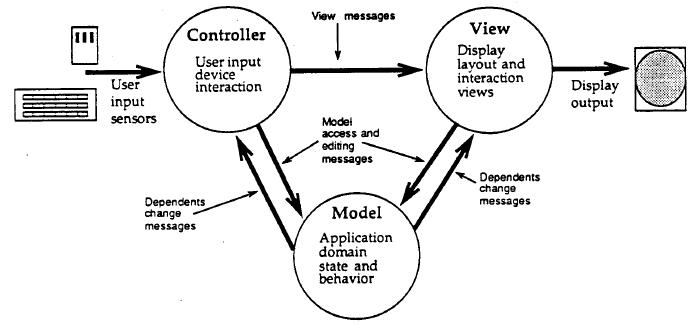
\includegraphics[scale=0.85]{krasner_mvc.jpg}
\caption{Model-View-Controller State and Message Sending \cite[s. 5]{krasner_desc}}
\end{figure} 
Jokaisella komponentilla on oma rajattu tehtävänsä ja ohjelmakoodi tulee jakaa näiden komponentien kesken. Jotta MVC:tä pystyttäisiin käyttämään
tehokkaasti, tulee ymmärtää komponenttien työnjako sekä se kuinka komponentit kommunikoivat keskenään \parencite{burbeck}. 

Luodessamme MVC-arkkitehtuurin toteuttavia komponentteja, tulee ne periä jostakin abstraktista pohjaluokasta (Model, View tai Controller), joka määrittelee kyseisen komponentin käyttäytymisen MVC:ssä  \parencite[s. 5]{krasner_desc}.  Tässä kappaleessa käydään jokaisen komponentin toteutus erikseen läpi käyttäen ohjelmointikielenä Smalltalkia. Lähteenä käytetään Krasnerin julkaisua \parencite{krasner_desc}.

Yleisesti MVC-komponenttien toimintaa kuvaavassa esimerkissä käyttäjältä tulee jokin syöte, jonka sillä hetkellä aktiivinen ohjain ottaa vastaan. Syötteen perusteella ohjain lähettää mallille viestin. Malli puolestaan tekee sille määrättyjä operaatioita muuttaen tilaansa ja lähettää edelleen viestin muutoksestaan kaikille siihen liitetyille riippuvuuksille (näkymät ja ohjaimet). Näkymät
voivat tämän jälkeen kysyä mallilta sen nykyistä tilaa ja päivittää itsensä, jos siihen on tarvetta. Ohjaimet voivat myös muuttaa tilaansa riippuen mallin tilasta \parencite[s. 4]{krasner_desc}. 

Suurin merkitys MVC:llä on luoda silta ihmismielen hahmottamalle mallille ja tietokoneessa esiintyvälle mallille. Oikein toteutettuna MVC:n avulla luodaan illuusio siitä, että käyttäjä kommunikoi suoraan mallin kanssa. Todellisuudessa kuitenkin ohjain ja näkymä muodostavat yhdessä rajapinnan sille, miltä malli näyttää ulospäin ja miten sitä käsitellään. Ohjain huolehtii syötteiden vastaanottamisesta ja käsittelemisestä. Näkymä taas huolehtii mallin graafisesta puolesta \parencite[s. 11-12]{reenskaug_tools}. 

\section{Historia}
MVC:n esitteli Norjalainen Trygve Reenskaug ollessaan mukana Xerox PARC -tutkimushankkeessa. 
Ensimmäinen julkaisu MVC:stä kirjoitettiin vuonna 1978 samassa tutkimuskeskuksessa. 
Tuolloin julkaisussa esiteltiin kolmen komponentin sijasta neljä komponenttia: 
Malli (Model), Näkymä(View), Ohjain(Controller) sekä Muokkaaja(Editor). Muokkaaja on 
väliaikainen komponentti, jonka näkymä luo itsensä ja syötelaitteiden välille. 
Muokkaaja-komponentista kuitenkin luovuttiin käsitteenä ja se sisällytettiin näkymään 
ja ohjaimeen \parencite{xerox}. Alkuperäinen Xerox PARC:n tuottama raportti MVC:stä oli Reenskaugin 
vuonna 1979 kirjoittama THING-MODEL-VIEW-EDITOR \parencite{xerox-thing}. Raportti esitteli MVC:n 
komponentteja käyttäen hyväksi esimerkkejä Reenskaugin omasta suunnittelutyöstä. Thing-komponentilla mallinnettiin
jotakin isompaa kokonaisuutta, joka hallitsee pienempiä kokonaisuuksia. Sitä voidaan ajatella eräänlaisena suurena mallina,joka on jaettu useisiin pienempiin malleihin. Editor-komponentti luo rajapinnan käyttäjän ja yhden tai useamman näkymän välille. Se tarjoaa käyttäjälle sopivan komento-rajapinnan kuten esimerkisi valikon, joka vaihtuu sisällön muuttuessa \parencite{xerox-thing}. Reenskaug hylkäsi kuitenkin Editor- ja Thing-komponentin ja  päätyi Adele Goldbergin avustuksella termeihin Models-Views-Controllers julkaisten saman vuoden lopulla raportin, jossa määritellään lyhyesti jokaisen komponentin tehtävä (MODELS-VIEWS-CONTROLLERS) \parencite{xerox-original}. Koska MVC:n historia ja suurin osa MVC:n alkuperäisistä julkaisuista pohjautuvat Smalltalk-ohjelmointikieleen, esitellään myös tässä tutkielmassa MVC:n totetusta Smalltalkilla.
Tämä ei kuitenkaan rajoita tarkastelua, koska arkkitehtuurin idea pysyy täysin samana riippumatta ohjelmointikielestä.

\section{Malli (Model)}
Malli pitää yllä sovelluksen tilaa sekä vastaa sovelluksen tallentamasta datasta. Se voi olla esimerkiksi kokonaislukumuuttuja laskuri-sovelluksessa, merkkijono-olio tekstinkäsittelyohjelmassa tai
mikä tahansa monimutkainen olio \parencite[s. 3]{krasner_desc}. Kaikkein yksinkertaisimmassa tapauksessa mallin ei tarvitse kommunikoida ollenkaan ohjaimen ja näkymän kanssa, vaan toimia passiivisena säiliönä datalle.
Tällaisesta tilanteesta on hyvä esimerkki yksinkertainen tekstieditori, jossa teksti nähdään juuri sellaisena kuin se olisi paperilla. Tässä tapauksessa mallin ei tarvitse ottaa vastuuta
kommunikoinnista näkymälle, koska muutokset tekstiin tapahtuvat käyttäjän pyynnöstä. Tällöin ohjain ottaa vastaan käyttäjän syötteet ja voi esimerkiksi ilmoittaa näkymälle muutoksesta, jolloin näkymä
päivittää mallin. Ohjain voi myös päivittää mallin ja ilmoittaa tästä näkymälle, jolloin näkymä voi pyytää mallin sen hetkistä tilaa. Kummassakaan tapauksesssa mallin ei tarvitse tietää ohjaimen ja näkymän
olemassaolosta \parencite{burbeck}.

Malli ei kuitenkaan aina voi olla täysin passiivinen. Se voi myös muuttua ilman, että se tarvitsee ohjaimen tai näkymän käskyä. Otetaan esimerkiksi malli, joka muuttaa tilaansa satunnaisin väliajoina. Koska malli muuttaa itseään, täytyy sillä olla jokin yhteys näkymään, jotta se voi antaa tiedon muutoksestaan \parencite{burbeck}. Datan kapseloinnin ja ohjelmakoodin uudelleen käytön kannalta ei ole kuitenkaan järkevää, että malli on suoraan yhteydessä näkymään ja ohjaimeen. Ohjaimen ja näkymän tulee siis olla riippuvaisia mallista, mutta ei toisinpäin. Näin mahdollistetaan myös se, että mallilla voi olla useita näkymiä ja ohjaimia \parencite[s. 4]{krasner_desc}.

Yleensä mallin tila muuttuu ohjaimista tulleiden käskyjen kautta. Tämän muutoksen tulisi heijastua kaikkiin näkymiin, jotka ovat sidottuja malliin. Tällaisia tilanteita varten kehitettiin riippuvuudet (\emph{dependents}).
Riippuvuuksilla tarkoitetaan listaa niistä ohjaimista ja näkymistä, jotka ovat sidottuja malliin. Mallilla tulee siis olla lista riippuvuuksista ohjaimiin ja näkymiin sekä myös kyky lisätä ja poistaa niitä. Malli ei siis tiedä mitään yksittäisistä riippuvuuksista, mutta pystyy kuitenkin lähettämään itsestään muutosviestejä (\emph{change messages}) listassa oleville ohjaimille ja näkymille. Mallin tuottamat muutosviestit voivat olla minkä tyyppisiä tahansa, joten ohjaimet ja näkymät reagoivat niihin omalla määritellyllä tavallaan  \parencite[s.2-3]{krasner}.

Mallille määritellään pääluokka \emph{Model} ja tälle viitemuuttuja \emph{dependents}, joka viittaa yhteen riippuvaan komponenttiin tai listaan riippuvista komponenteista. Kaikki uudet mallit tulee periä niiden pääluokasta, jotta saavutetaan sama toiminnallisuus kaikkiin mallikomponentteihin. Komponenttien tieto mallin muutoksista tukeutuu täysin mallin riippuvuusmekanismiin. Kun jokin komponentti luodaan, se rekisteröi itsensä malliin riippuvuudeksi ja samalla tavalla se myös poistaa itsensä \parencite{burbeck}. Näkymät käyttävät riippuuvuusmekanismia päivittääkseen itsensä mallin muutoksien perusteella. Esimerkiksi mallin muuttuessa lähetätetään \textit{changed}, jonka pohjalta jokainen riippuvuus saa \textit{update} -viestin.Viestillä voi olla myös erilaisia parametrejä, joiden perusteella viestiä pystytään tarkentamaan. Esimerkiksi mallin, johon on liitetty useita näkymiä, ei välttämättä tarvitse lähettää kaikille näkymille viestiä muutoksestaan. Se voi välittää viestin mukana parametrina tiedon muutoksesta, jonka perusteella jokainen vastaanottaja voi päättää miten toimia \parencite{burbeck}.

Alkuperäinen \textit{update} -metodi on peritty \textit{Object} -luokasta, eikä se tuolloin tee vielä yhtään mitään. Useimmilla näkymillä se on kuitenkin toteutettu näyttämään näkymä uudestaan kutsuttaessa. Tämä \textit{changed/update} -mekanismi valittin toimimaan kommunikaatiokanavana mallien ja näkymien välille, koska se aiheuttaa vähiten rajoituksia ja esteitä \parencite{burbeck}. 

\subsection{Näkymä (View)}
Näkymän tehtävänä on huolehtia graafisesta puolesta MVC:ssä. Näkymä pyytää yleensä mallilta datan ja tämän pohjalta näyttää käyttäjälle käyttöliittymän sovellukseen. Toisinkuin malli, jota pystytään rajoittamattomasti yhdistelemään moniin näkymiin ja ohjaimiin, jokainen näkymä on liitetty yhteen ohjaimeen.  Näkymä siis sisältää viitteen ohjaimeen ja ohjain sisältää viitteen näkymään. Kuten ohjain, näkymä on myös rekisteröity mallin riippuvuuksiin. Kummatkin sisältävät siis myös viitteen siihen malliin, johon ne on rekisteröity \parencite{burbeck}. Jokaisella näkymällä on tasan yksi malli ja yksi ohjain \parencite[s. 7]{krasner_desc}.

Näkymä vastaa myös MVC-komponenttien sisäisestä kommunikaatiosta MVC-kolmikon luontivaiheessa. Näkymä rekisteröi itsensä  riippuvuudeksi malliin, asettaa viitemuuttujansa viittamaan ohjaimeen ja välittää itsestään viestin ohjaimelle. Viestin avulla ohjain rekisteröi näkymän omaan viitemuuttujaansa. Näkymällä on myös vastuu poistaa viitteet sekä rekisteröinnit \parencite{burbeck}. 

Näkymä ei sisällä ainoastaan komponentteja datan näyttämiseen ruudulla, vaan se voi sisältää myös useita alanäkymiä (\emph{subviews}) ja ylänäkymiä (\emph{superviews}). Tästä muodostuu hierarkia, jossa ylänäkymä hoitaa aina jonkun suuremman kokonaisuuden, kuten esimerkiksi näytön pääikkunan. Alanäkymä taas huolehtii jostain pienemmästä yksityiskohdasta pääikkunassa. Näkymillä on myös viite erilliseen transformaatioluokkaan, joka hoitaa kuvan sovittamisen ja yhdistämisen alanäkymien ja ylänäkymien välillä. Jokaisella näkymällä tulee siis olla toteutus, jolla hoidetaan alanäkymien poistaminen sekä lisääminen. Samalla tulee määritellä ominaisuus, jolla sisäiset transformaatiot tuodaan transformaatioluokalle. Tämä helpottaa näkymän ja sen alanäkymien yhdistämistä \parencite[s. 8]{krasner_desc}. Burbeck havainnollistaa Smalltalkilla kirjoitetulla esimerkillä kuinka MVC-kolmikko luodaan. Esitetyssä esimerkissä on yksinkertaistettu versio MVC-kolmikon luonnista siten, että mukana on myös ylä- ja alanäkymien toteutus.

\begin{lstlisting}[language=Smalltalk]
openListBrowserOn: aCollection label: labelString initialSelection: sel
  "Create and schedule a Method List browser for 
  the methods in aCollection."
  | topView aBrowser | 
  aBrowser := MethodListBrowser new on: aCollection.
  topView := BrowserView new.
  topView model: aBrowser; controller: StandardSystemController new;
                 label: labelString asString; minimumSize: 300@100.
topView addSubView:
  (SelectionInListView on: aBrowser printItems: false oneItem: false
  aspect: #methodName change: #methodName: list: #methodList
  menu: #methodMenu initialSelection: #methodName)
  in: (0@0 extent: 1.0@0.25) borderWidth: 1.
topView addSubView:
  (CodeView on: aBrowser aspect: #text change: #acceptText:from:
  menu: #textMenu initialSelection: sel)
  in: (0@0.25 extent: 1@0.75) borderWidth: 1.
  topView controller open
\end{lstlisting}

Seuraavaksi käydään rivi kerrallaan läpi mitä yllä esitetyssä ohjelmakoodissa tapahtuu. Mallin luonnin jälkeen [5] luodaan viite uudelle \textit{BrowserView} -luokan instanssille [6]. \textit{BrowserView} on peritty \textit{StandardSystemView} -luokasta. Seuraavaksi määritellään malli ja ohjain sekä muuttujat näkymän otsikolle ja koolle [7]. Jos ohjainta ei määritellä erikseen, käytetään näkymän \textit{defaultController} metodia. Riveillä [7-11] luodaan alanäkymä \textit{SelectionInListView} ja riveillä [12-15] luodaan toinen alanäkymä \textit{CodeView}. Lopuksi [16] avataan ohjain, joka käynnistää ikkunoiden piirtämisprosessin.

Näkymät saattavat tarvita myös oman protokollan itsensä näyttämiseen. Kun malli ilmoittaa muutoksestaan, \textit{update} -metodi näkymässä kutsuu \textit{display}, joka puolestaan kutsuu \textit{displayBorder}, \textit{displayView} ja \textit{displaySubviews}. Jos näkymä tarvitsee erityistä käyttäytymistä itsensä näyttämiseen, se toteutetaan edellämainituissa metodeissa. Muuten käytetään pääluokasta perittyjä ominaisuuksia \parencite{burbeck}. Monet näkymät käyttävät myös erilaisia transformaatio-instansseja, joilla hallitaan esimerkiksi näkymän skaalausta ruudulla. Tähän ei kuitenkaan perehdytä sen enempää, koska ne menevät tutkimuksen rajojen ulkopuolelle.


\subsection{Ohjain (Controller)}
Ohjaimen tehtävänä on ottaa vastaan syötteitä sekä koordinoida malleja ja näkymiä saatujen syötteiden perusteella. Sen tulee myös kommunikoida muiden ohjaimien kanssa. Teknisesti ohjaimessa on kolme viitemuuttujaa: malli, näkymä ja sensori (sensor). Sensorin tehtävänä on toimia rajapintana syötelaitteiden sekä ohjaimen välillä. Sensori mallintaa syötelaitteiden käyttäytymistä ja muuttaa ne ohjaimen ymmärtämään muotoon.

Ohjaimien tulee käyttäytyä siten, että vain yksi ohjain ottaa vastaan syötteitä kerrallaan. Esimerkiksi näkymät pystyvät esittämään informaatiota rinnakkain monen näkymän kautta, mutta käyttäjän toimintoja tulkitsee aina vain yksi ohjain. Ohjain on siis määritelty käyttäytymään siten, että se osaa tietyn signaalin perusteella päättää tuleeko sen aktivoida itsensä vai ei. Ohjain sisältää toiminnallisuuden jonka perusteella se pystyy päättämään tuleeko hallinta pitää itsellä vai luovuttaa eteenpäin \parencite[s. 9]{krasner_desc}. Ohjainten ylimmällä tasolla on \textit{ControlManager}, joka kysyy jokaiselta päänäkymään liitetyltä ohjaimelta erikseen, haluaako tämä ottaa hallinnan. Jos ohjaimen näkymä sisältää kursorin, vastaa ohjain kutsuun myönteisesti, jolloin kyseinen ohjain saa hallinnan. Hallitsevan ohjaimen näkymä kysyy seuraavaksi mahdollisten alanäkymien ohjaimilta samalla tavalla haluaako jokin ohjaimista hallinnan itselleen. Jos myönteisesti vastaava ohjain löytyy, ottaa se uuden hallinnan. Tätä prosessia jatkamalla löydetään matalimman tason näkymä ja sen ohjain ottaa lopullisen hallinnan. Ohjain pitää hallinnan itsellään niin kauan kunnes kursoria liikutetaan näkymän rajoista ulos. Ainoastaan se jonka kohdalla kursori on, vastaa kutsuun ja tuolloin ottaa hallinan. Näkymillä on oikeus kysyä alanäkymiensä ohjaimia. Ohjaimien tehtävänä on kysyä omalta näkymältään onko kursori niiden päällä.

Krasner määrittelee seuraavat metodit, joiden avulla ohjaimet viestivät \parencite[s. 9]{krasner_desc}:

\begin{description}
\item[isControlWanted] -\ Tuleeko ohjaimen ottaa hallinta.
\item[isControlActive] -\ Onko ohjain aktiivinen.
\item[controlToNextLevel] -\ Luovutetaan hallinta seuraavalle ohjaimelle.
\item[viewHasCursor] -\ Onko ohjaimen näkymässä hiiren kursori.
\item[controlInitialize] -\ Kun ohjain on saanut hallinnan, alustetaan se.
\item[controlLoop] -\ Lähettää \emph{controlActivity} -viesteja niin kauan, kuin ohjaimella on hallinta.
\item[controlTerminate] -\ Lopettaa ohjaimen hallinnan.
\end{description} 

Kun ohjain saa hallinnan itselleen, kutsuu se \emph{startUp} -metodia, joka puolestaan kutsuu seuraavia metodeja: \emph{controlInitialize}, \emph{controlLoop} ja \emph{controlTerminate}. Metodit
voidaan ylikirjoittaa, jolloin saavutetaan jokin haluttu ominaisuus kyseisessä vaiheessa. Esimerkiksi \emph{controlInitialize} ja \emph{controlTerminate} määräävät mitä tehdään, kun ohjain saa hallinnan tai luovuttaa sen eteenpäin. Ohjaimen hallinnan aikana kutsutaan
\emph{controlLoop} -metodia, joka taas kutsuu \emph{controlActivity} -metodia niin kauan kuin ohjaimella on hallinta.  Metodi \emph{controlActivity} määrää ohjaimen toiminnan hallinnan aikana \cite[s. 9]{krasner_desc}.

\subsection{Esimerkkiohjelma}
Seuraavaksi esitellään  Dortmundin yliopistossa kirjoitettu yksinkertainen esimerkkiohjelma Smalltalkilla siitä miten MVC:n toteutus tuodaan sovellukseen käytännössä. Ohjelmakoodi löytyy myös Krasnerin artikkelista \cite[s. 20]{krasner_desc}. Ohjelmassa toteutetaan yksinkertainen laskuri-ohjelma, joka käyttää MVC-arkkitehtuuria toteutuksessaan. Ohjelmassa esitellään mallina \emph{Counter} -luokka ja näkymänä \emph{CounterView} -luokka. \emph{Counter} perii mallin ominaisuudet ja
toimii ohjelmassa yksinkertaisen kokonaisluku-muuttujan ylläpitäjänä. \emph{CounterView} perii näkymän ominaisuudet ja esittää mallin arvon ruudulla.
Ohjaimena toimii \emph{CounterController} -luokka, joka perii ohjaimen käyttäytymisen. Ohjain tarjoaa sovellukselle painikkeet, joista voidaan vähentää
tai lisätä laskurin arvoa.

Määritellään ensiksi \emph{Counter} -luokka, joka peritään \emph{Model} -luokasta.
\begin{lstlisting}[language=Smalltalk]
Model subclass: #Counter
	instanceVariableNames: 'value'
	classVariableNames: ''
	poolDictionaries: ''
  	category: 'Demo-Counter'
\end{lstlisting}
Seuraavaksi määritellään \emph{Counter}-luokalle metodeita, jotka määrävät
laskuriarvon alustamisen sekä muokkaamisen.
\begin{lstlisting}[language=Smalltalk]
Counter methods For: 'Initialize-release'
Initialize
	"Aseta alkuarvoksi 0"
	self value: 0
Counter methodsFor: 'accessing'
value
	"Palauta mallin arvo"
   	^value
value: aNumber
	"Aseta mallin arvo"
	value <- aNumber.
	self changed "to update displayed value"
Counter methodsFor: 'operations'
decrement
	"Vähennä mallin arvoa yhdellä."
	self value: value -1
Increment
	"Lisää mallin arvoa yhdellä."
	self value: value + 1
\end{lstlisting}
Lisätään luokkaan metodi, jolla itse luokasta saadaan muodostettua instanssi.
\begin{lstlisting}[language=Smalltalk]
Counter class methodsFor: 'instance creation'
new
	"Palauta uusi instanssi luokasta"
	^super new initialize
\end{lstlisting}
Seuraavaksi määritellään ohjain (\emph{CounterController}), joka peritään
\emph{Controller} luokasta. Luodaan myös ohjaimelle metodit, joiden avulla
ohjataan mallia sekä näkymää. Metodeissa toteutetaan valikko, joka tarjoaa
mahdollisuuden joko vähentää tai lisätä laskurin arvoa. Kaikki \emph{CounterController} -luokassa käytetyt
määrittelemättömät muuttujat peritään yliluokasta.
\begin{lstlisting}[language=Smalltalk]
Mouse MenuController subclass: #CounterControIler
	instanceVariableNames: ' '
  	classVariableNames: ' '
  	poolDictionaries: ' '
  	category: 'Demo-Counter'
CounterController methodsFor: 'initialize-release'
initialize
	"Alusta valikko, jossa on mahdollisuus vähentää tai 
        lisätä mallin arvoa"
  	super initialize.
  	Self yellowButtonMenu: (PopUpMenu labels: 
                                  'Increment\Decrement' withCRs)
  	yellowButtonMessages: #(increment decrement)
CounterController methodsFor: 'menu messages'
decrement
	"Vähennä mallin arvoa yhdellä."
 	self model decrement
increment
	"Lisää mallin arvoa yhdellä"
	self model increment
CounterController methodsFor: 'control defaults'
isControlActlve
	"Ota hallinta kun sinistä nappia ei paineta"
	^super isControlActive & sensor blueButtonPressed not
\end{lstlisting}
Määrätään näkymä (\emph{CounterView}), joka peritään \emph{View} -yliluokasta. Määrätään
myös näkymälle metodit, joiden avulla näytetään mallin tila ruudulla.
\begin{lstlisting}[language=Smalltalk]
View subclass: #Counterview
	instanceVariableNames: ''
	classVariableNames: ''
	poolDictionaries: ''
	category: 'Demo-Counter'

CounterView methodsFor: 'displaying'
displayView
	"Näytä mallin arvo näkymässä"
	| box pos displayText |
	box := self insetDisplayBox.
	"Asettele teksti näkymään. Asettelu ei
	 ole tutkielman kannalta oleellista."
	pos := box origin + (4 @ (box extent y / 3)).
	displayText := ('value:', self model value printString)
					asDisplayText.
	displayText displayAt: pos
\end{lstlisting}
Määritellään \emph{update} -metodi, jotta näkymä pystyy päivittämään itsensä. Metodia kutsutaan
yleensä mallin tilan muuttuessa.
\begin{lstlisting}[language=Smalltalk]
CounterView methodsFor: 'updating'
update: aParameter
  "Yksinkertaisesti päivitä näyttö uudestaan"
  self display
\end{lstlisting}
Luodaan myös metodi, joka palauttaa näkymään liitetyn ohjaimen.
\begin{lstlisting}[language=Smalltalk]
CounterView methodsFor: 'controller access'
defaultControllerClass
	"Palauta näkymään rekisteröity ohjain"
	^CounterController
\end{lstlisting}
Lopuksi tarvitaan metodi, joka luo uuden näkymän sekä rekisteröi mallin ja ohjaimen itseensä. Näkymä näyttää ruudulta
samalta kuin kuvassa 2.
\begin{lstlisting}[language=Smalltalk]
CounterView class methodsFor: 'instance creation'
open
	"Avaa näkymän uudelle laskurisovellukselle. Tässä 
	metodissa nähdään kuinka näkymä huolehtii mallin 
	rekisteröinnistä sekä nähdään kuinka näkymiä voi 
	olla useita sisäkkäin."
	| aCounterView topView |
	"Luo laskurinäkymälle uusi näkymä, joka näyttää 
	laskurin arvon"
	aCounterView := CounterView new
	"Asetetaan malliksi Counter -luokan instanssi"
	model: Counter new.
	aCounterView borderWidth: 2.
	aCounterView insideColor: Form white.
	"Asetetaan ylimmäksi näkymäksi StandardSystemView 
	-luokan instanssi, joka vastaa perinteistä
ikkunointimallia"
	topView := StandardSystemView new
		label: 'Counter'.
	topView minimumSize: 80@40.
	"Lisätään edellä luotu laskurinäkymä ylinäkymän 
	alanäkymäksi"
	topView addSubView: aCounterView.
	"Käynnistetään ohjain"
	topView controller open
\end{lstlisting}

\begin{figure}[h]
\centering
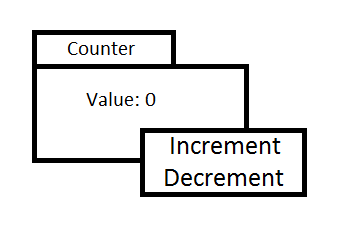
\includegraphics[scale=0.85]{counter.png}
\caption{Kuva CounterView -näkymästä \cite{krasner_desc}}
\end{figure}

\section{Pyramid}
Pyramid on Python-pohjainen web-sovelluskehys, jonka tehtävänä on helpottaa web-kehitystä tarjoamalla
kehittäjälle valmiita työkaluja avuksi kehitykseen.

\subsection{Tausta}
Sovelluskehyksen tehtävänä on tuoda sovelluksen kehitykseen mukaan
taso, joka tarjoaa erilaisia kirjastoja ratkaisemaan yleisimpiä ongelmia, joita tulee vastaan sovelluksen kehityksen aikana. Näin vältetään
jo ratkaistujen perusoperaatioiden toistoa ja pystytään keskittymään suoraan sovelluksen toteuttamiseen. Web"-sovelluskehykset ovat erityisesti suunnattuja
web-sovellusten ja -palvelujen toteuttamiseen.  Tärkein ero sovelluskehyksen ja kirjaston välillä on se, että kirjaston ohjelmakoodi kutsustaan aina
kehittäjän toimestaa. Sovelluskehyksessä taas kehittäjän ohjelmakoodia kutsutaan aina sovelluskehyksen toimesta \cite{Pyramid:intr}.

\chapter{Sovelluskehykset}
Soveluskehykset ovat suosittuja, koska ne tarjoavat uudelleenkäytettäviä ratkaisuja erilaisiin ongelmiin sovelluskehityksessä. Toimialueesta riippumatta sovelluskehyksiä tulisi käyttää hyväksi kirjottaessa monimutkaisia sovelluksia. Sovelluskehys tuo sovellukseen tason, jossa sovelluksen osat on abstrahoitu erilaisilla luokilla sekä rajapinnoilla, joita voidaan käyttää uudelleen sovelluksen eri osissa. Sovelluskehys ei ole vain kokoelma rajapintoja ja kirjastoja\parencite{towards_framework}. Tärkein ero sovelluskehyksen ja kirjaston välillä on se, että kirjaston ohjelmakoodi kutsustaan aina
kehittäjän toimestaa. Sovelluskehyksessä taas kehittäjän ohjelmakoodia kutsutaan aina sovelluskehyksen toimesta \parencite{pyramid_intr}.

Sovelluskehys ei myöskään generoi koodia. Se käyttää erilaisia komponentteja ja kirjastoja luodakseen infrastruktuurin, jonka päälle voidaan rakentaa sovelluksia sovelluskehyksen ehdoilla. Sovelluskehyksen käyttäminen myös rajoittaa sovelluksen rakennetta ja pakottaa sovelluksen toteuttamaan asioita tietyin ehdoin. Rajoitusten ansiosta sovelluskehittäjä voi keskittyä toimialueeseen liittyviin ongelmiin välittämättä koko sovelluksen yksityiskohtaisesta toteutuksesta \parencite{towards_framework}.

Web-sovelluskehykset ovat sovelluskehyksiä, jotka tarjoavat ratkaisuja helpottamaan web-sovellusten toteuttamista. Web-sovelluskehyksissä käyttöliittymä näytetään käyttäjille selaimen välityksellä. Sovellus ajetaan joko serverillä tai suoraan käyttäjän selaimessa. Sovellus määrittää käyttöliittymän sivujen järjestyksen, sisällön sekä mahdollisten toimintojen esittämisen käyttäjälle, jonka kautta käyttäjä voi vaikuttaa serverillä sijaitsevaan sovellukseen \parencite{vosloo}.

Web-sovelluskehykset voidaan jakaa serveri-pohjaisiin ja selain-pohjaisiin sovelluskehyksiin. Serveri-pohjaisissa web-sovelluskehyksissä sovelluksen tilaa hallitaan serverin puolella. Tuolloin käyttöliittymää perustuu tilaan, mikä on sillä hetkellä serverin puolella. Selain-pohjaisissa sovelluskehyksissä sisältö muuttuu selaimen sisällä käyttäjän päässä \parencite{vosloo}. Tässä tutkimuksessa käsiteltävät sovelluskehykset ovat Pythonilla toteutettuja serveri-pohjaisia sovelluskehyksiä.

\section{Pyramid}

Pyramid on Python-pohjainen web-sovelluskehys, jonka tehtävänä on helpottaa web-kehitystä tarjoamalla
kehittäjälle valmiita työkaluja avuksi kehitykseen. Pyramid on suunniteltu siten, että kehittäjän ei tarvitse tietää suuria määriä erilaisia malleja ja tekniikoita pystyäkseen tuottamaan web-sovelluksia. Se ei myöskään pakota käyttämään kehityksessä mitään erityistä tekniikkaa, vaan pyrkii olemaan mahdollisimman yksinkertainen ja helposti laajennettavissa erilaisiin käyttötarkoituksiin. Laajentamisella tarkoitetaan erilaisten lisäosien liittämistä Pyramidiin. Yksinkertaisuuden ja mimimaalisuuden ansiosta se on myös nopeampi kuin monet muut Python-pohjaiset web-sovelluskehykset. Tämä johtuu Pyramidin poikkeuksellisen pienestä kutsupinosta ajamisen aikana \parencite{pyramid_intr}. 

Pyramid sai alkunsa Pylons -projektista syyskuussa vuonna 2005, jolloin jo yli 30 Python-sovelluskehystä kilpaili käyttäjistä. Ben Bangert ja James Gardner alkoivat yhdessä kehittää sovelluskehystä, josta tuli lopulta Pylons. Alunperin Pylons oli
muokattu Myghty Python Templating Framework:n pohjalta tarjotakseen MVC-pohjaisen web-sovelluskehyksen. Myghty -sovelluskehystä ajettiin mod\_pythonin päällä, mutta Pylonsin pyrkimys oli käyttää WSGI:tä hyödyntämään joustavaa komponenttipohjaista lähestymistapaa web-sovelluksissa \parencite{pyramid_history}. Pylons projektin tarkoituksena ei ole keskittyä yhden yksittäisen web-sovelluskehyksen kehittämiseen vaan tarjota kokoelma erilaisia teknologioita \parencite{pylons_about}. Vuonna 2008 Pyramid tunnettiin nimellä repoze.bfg. Joulukuun alussa tapahtui ohjelmakoodin uudelleen nimeäminen ja ominaisuuksien lisääminen sekä poistaminen \parencite{pyramid_about}.


Koska Pyramid pyrkii tarjoamaan vain välttämättömimmät työkalut web"-sovelluksien kehitykseen, sen kehittäjät
ovat päätyneet web-kehityksessä neljään yleisimpään ongelmaan ja tarjoavat niihin ratkaisun Pyramidissa:

\begin{description}
\item [URL Mapping] -\ URL:ien liittäminen ohjelmakoodiin.
\item[Template] -\ Tuodaan sovelluksen näkymä selaimelle käyttäen HTML-kieltä, jolla määrätään näkymän rakenne. Tämän avulla pystytään erottamaan käyttöliittymä sovelluslogiikasta tehokkaasti.
\item[Security] -\ Perinteiset tietoturvaongelmat tulee olla ratkaistuna valmiiksi jo sovelluskehyksessä. Tämä ei kuitenkaan tarkoita sitä, että kehittäjä voisi täysin unohtaa tietoturvan merkityksen.
\item[Static Assets] -\ Staattisien resurssejen jakaminen niille tarkoitettuihin paikkoihin tiedostorakenteessa.
\end{description}
Yllä määriteltyjen neljän ongelman lisäksi Pyramid tarjoaa lisäosien kautta monia erilaisia työkaluja, joiden avulla pystytään laajentamaan sen ominaisuuksia \parencite{pyramid_intr}. Tutkielman aiheen rajauksen vuoksi ei kuitenkaan
käydä läpi yksityiskohtaisemmin Pyramidin toteutusta ja siihen liitettävissä olevia lisäosia, vaan keskitytään tarkastelemaan MVC:n toteutusta Pyramidissa.

\section{Django}
Django luotiin palvelemaan tarkoitusta  World Online -verkkolehdelle, jonka tehtävänä oli rakentaa web-sovelluksia mahdollisimman nopeasti julkaisuja varten. 2003 World Online:n kehittäjät Adrian Holovaty ja Simon Willison aloittivat käyttämään Pythonia web-sivujen kehittämisessä. 

\section{Plone}
\section{Flask}

\chapter{MVC:n toteutus web-sovelluskehyksissä}
\section{Yleistä}
\section{Pyramid}
Pyramid väittää olevansa mvc-kehys
\section{Django}
django väittää olevansa mvc-kehys
\section{Plone}

\chapter{MVC and Flask}
\section{Esimerkkiohjelma}
\section{Pohdinta}
\section{Yhteenveto}

\chapter{Johtopäätökset}
\chapter{Tutkielman rakenne}
\section{Teoriaosa}
\section{Teorian jälkeen}
\chapter{Lähteiden käyttö}
\section{Lähdeviittaukset}

\printbibliography

\end{document}
